\documentclass[final, unknownkeysallowed]{beamer}
\usetheme{RJH}
\usepackage[orientation=portrait,size=a0,scale=1.0,debug]{beamerposter}
\usepackage[absolute,overlay]{textpos}
\usepackage{subcaption}
\captionsetup[subfigure]{labelformat=parens}
\setlength{\TPHorizModule}{1cm}
\setlength{\TPVertModule}{1cm}

\title{Deep convolutional networks for protein structure quality assessment}
\author{Georgy Derevyanko\inst{1}, Sergei Grudinin\inst{2}, Guillaume Lamoureux\inst{1}}
\institute[shortinst]{ \hspace{2cm}{\small \inst{1} Department of Chemistry and Biochemistry and Centre for Research in Molecular Modeling (CERMM), Concordia University, Montr{\'e}al, Canada \hspace{2cm}
\inst{2} NANO-D, INRIA Rhone-Alpes Research Center, Grenoble, France}}
\footer{}
\date{\today}

\makeatletter
\newcommand\nocaption{%
    \renewcommand\p@subfigure{}
    \renewcommand\thesubfigure{\thefigure\alph{subfigure}}
}
\makeatother


\begin{document}
\begin{frame}{}

\begin{textblock}{6}(64.5,0.5)

\includegraphics[width=10.0cm]{Logo/ConULogo_K}
\end{textblock}
\begin{textblock}{6}(76.,0.2)

\includegraphics[width=7.0cm]{Logo/CERMM_transparent.png}
\end{textblock}



\begin{textblock}{39.0}(2,6)
\begin{block}{Introduction}
Protein structure prediction remains one of the outstanding challenges
in structural biology.  Progress in this field is assessed during the
biennial CASP competition \cite{moult2014critical}, in which
contestants are given the sequences of a number of proteins for which
structures are about to be solved, and are attempting to predict their
structures.

\vspace{0.5cm}
A key part of all prediction pipelines competing in CASP is the decoy
quality assessment (QA). During this step, an algorithm selects the
best structure out of a pool of computer-generated candidate
structures (``decoys''). The final success of a prediction method
largely depends on the performance of the QA step.

\vspace{0.5cm}
In this work we propose an algorithm that learns the ranking of
protein candidate structures using only atomic densities. The key
advantages of our algorithm are:
\begin{itemize}
\item \emph{It avoids feature engineering.} Standard approaches use a
  pre-engineered set of features, fed to a machine learning model or
  an optimization algorithm.  However, the process of obtaining these
  features can be tedious and time-consuming.  Moreover, any list of
  features extracted from raw structural data is by definition
  incomplete and excludes potentially useful information. Our
  algorithm predicts the score of a decoy based only on the atomic
  densities.
\item \emph{It can learn from any type of spatial data.}
  Electrostatics and solvent are extremely important for protein
  stability.  However, this information is not directly accessible to
  current state-of-the-art QA methods.  Our approach enables
  straightforward access to any physical property defined in 3D space,
  such as atomic/electronic densities, electrostatic potential,
  solvent distribution, etc.
\end{itemize}
\end{block}

\begin{block}{Input and model}

The input of the model is a set of atomic densities. We assign atomic
types to each heavy atom of the structure, then we project the density
of each atom to the grid corresponding to its atom type (see
Fig.~\ref{Fig:atomic_densities}).  The density of each atom is
represented as a Gaussian.  The atom types are inspired by the SYBYL
classification.

\vspace{0.5cm}
We use 3D convolutional neural networks to predict the quality of a
candidate protein structure.  The schematic representation of the
model architecture is presented below (Fig.~\ref{Fig:CNNModel}).

\begin{figure}[H]
    \centering
    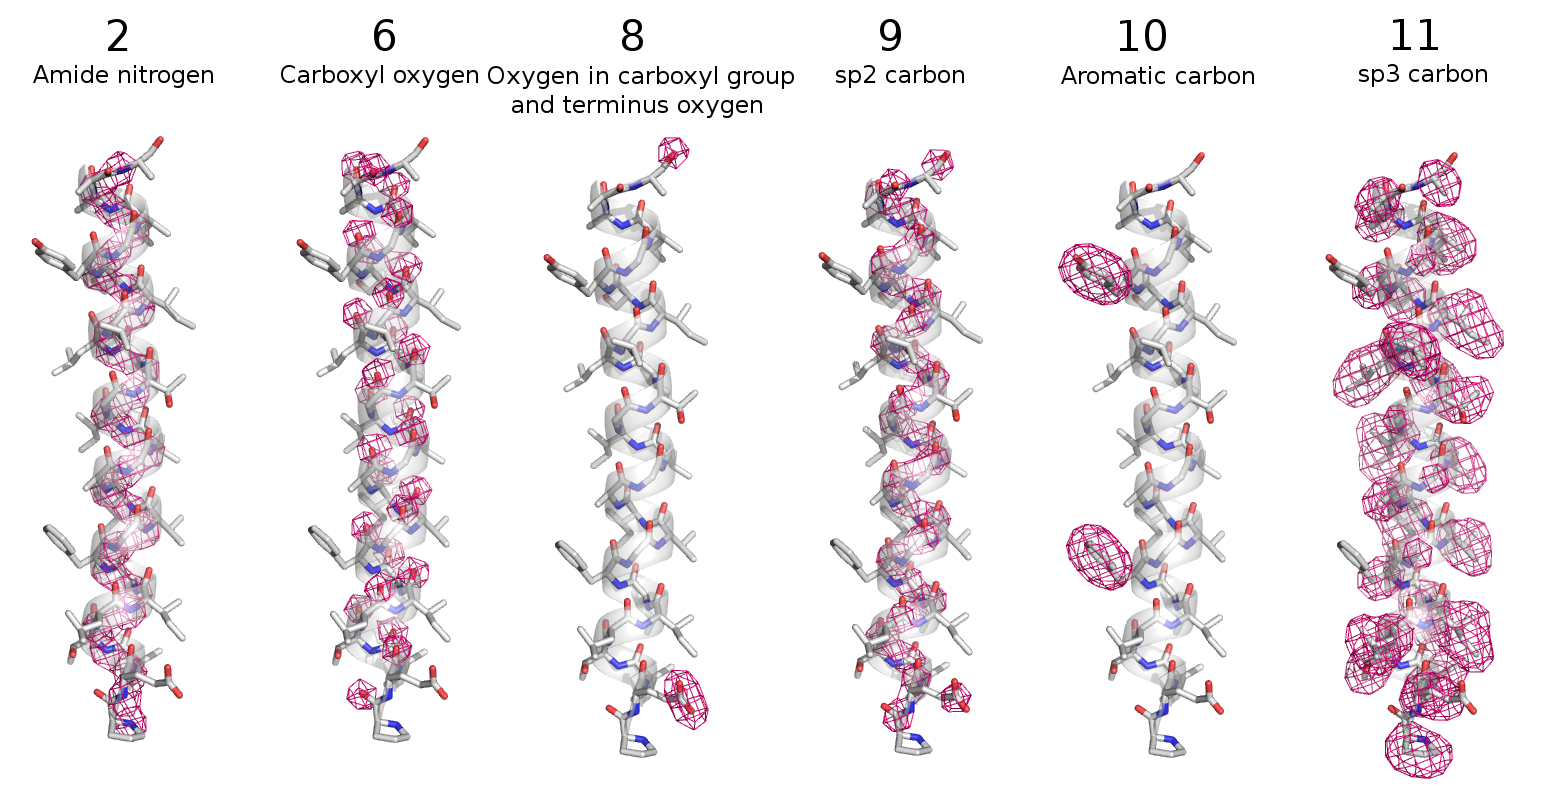
\includegraphics[width=0.6\linewidth]{../draft/Fig/atomic_densities_V3.png}
    \captionsetup{width=0.8\linewidth}
    \caption{Example of the representation of a protein structure
      using atomic densities. The density maps are represented by
      isosurfaces at the half-maximum level.}
    \label{Fig:atomic_densities}
\end{figure}

\begin{figure}[H]
    \centering
    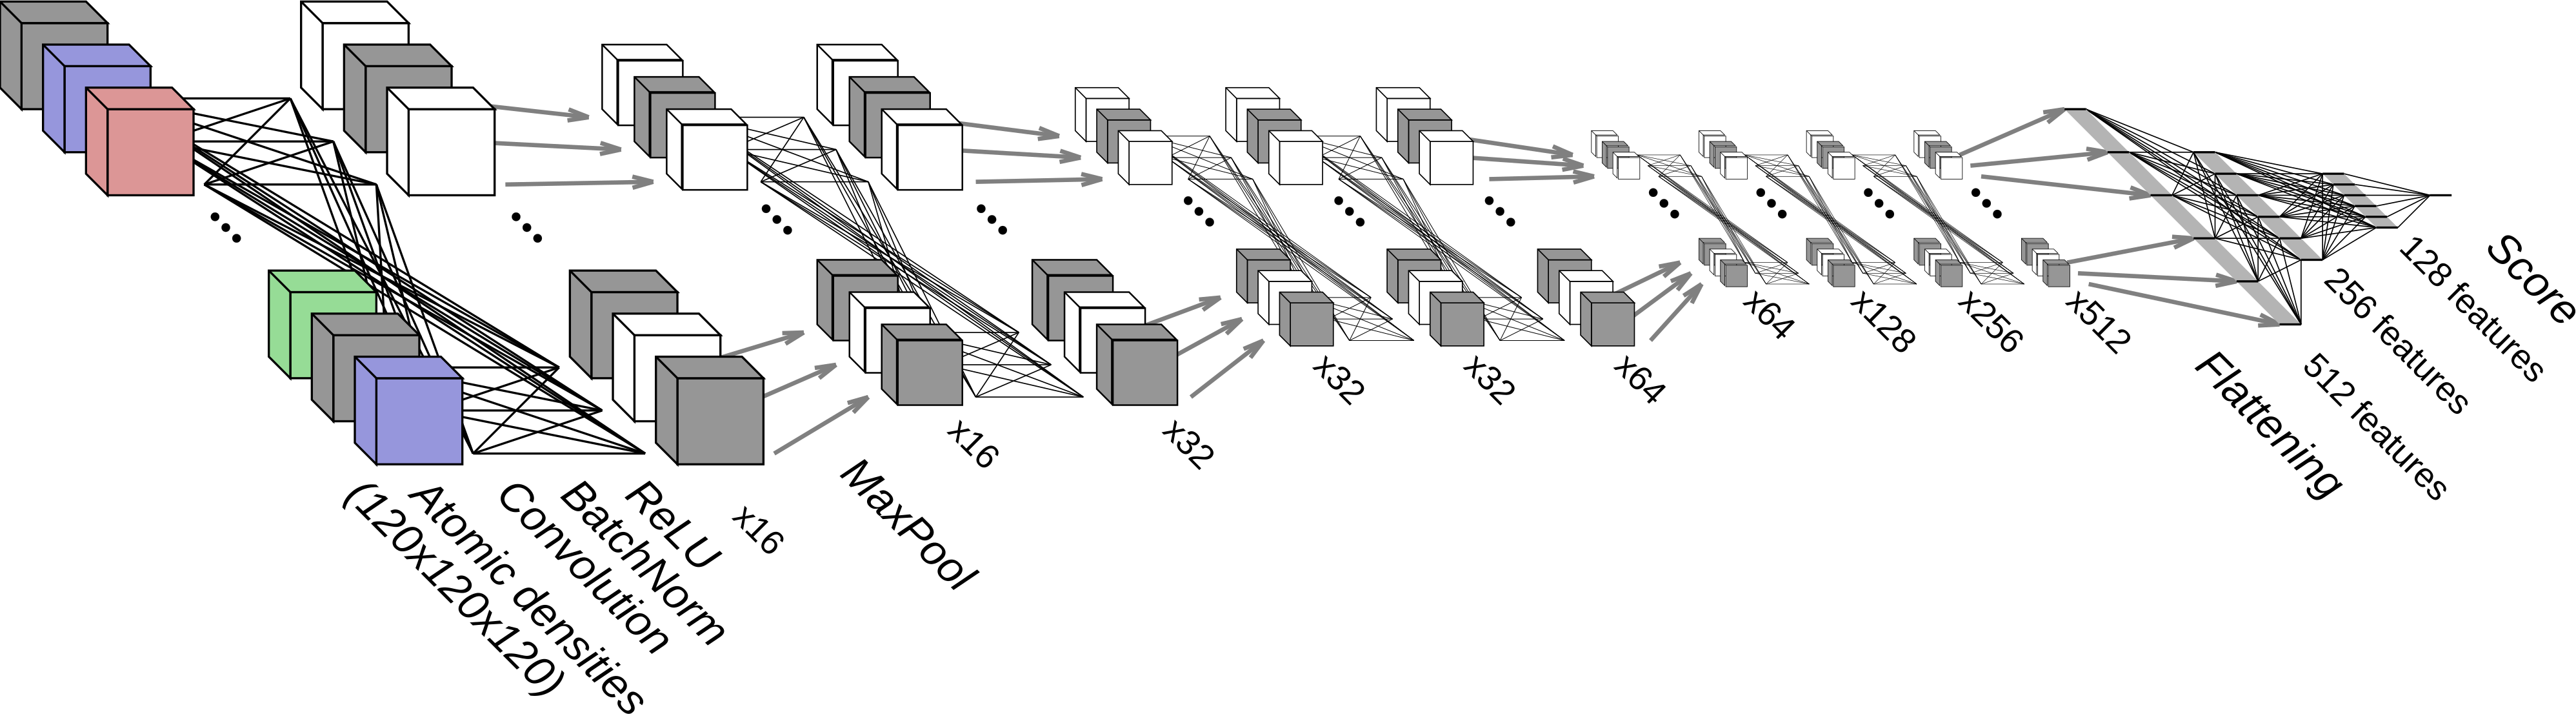
\includegraphics[width=\linewidth]{../draft/Fig/ConvnetDiagramV1.png}
    \captionsetup{width=0.8\linewidth}
    \caption{Convolutional neural network used in this work. Line
      connections across boxes denote the consecutive application of a
      3D convolutional layer, a batch normalization layer, and a ReLU
      layer. Arrows between boxes denote maximum pooling layers. The
      labels ``$\times M$'' denote the number of filters used in the
      corresponding 3D convolutional layer.}
    \label{Fig:CNNModel}
\end{figure}

We train the model to minimize the ranking loss function.  The ranks
for the decoys in the training dataset are defined using precomputed
GDT\_TS scores.  In particular, we use the pairwise ranking loss:
$$
L_{ij} = w_{ij} \cdot \max \left[ 0, 1 - y_{ij} \left( f(x_i) - f(x_j) \right) \right]
$$
where $w_{ij}$ is zero when the two decoys have too similar scores and is one
otherwise.  The $y_{ij}$ coefficients define the score ordering:
$$
y_{ij} = \begin{cases}
                1& \text{if } \textrm{GDT\_TS}_i \leq \textrm{GDT\_TS}_j \\
               -1& \text{if } \textrm{GDT\_TS}_i > \textrm{GDT\_TS}_j \\
           \end{cases}
$$
%During the training procedure, we optimize the loss function with
%respect to the parameters of the model.

\end{block}

\begin{block}{Datasets}

We train and assess our method using the decoys from previous CASP
competitions. We use the submissions from contestants of the CASP7 to
CASP10 competitions as training set and the decoys from the CASP11
competition as test set.
\begin{itemize}
\item The side chains of all structures from the training and test
  sets are optimized using SCWRL4 \cite{krivov2009improved}.
\item The training and test sets have 564 and 83 targets
  correspondingly. Each target in the training dataset has on average
  282 decoys.
\item The test dataset is split into two subsets: Stage 1 with 20
  selected decoys for each target and Stage 2 with 150 decoys for each
  target.
\item The native structures are excluded from both the training and
  test datasets, and are used only to precompute the GDT\_TS scores.
\end{itemize}

\vspace{0.5cm}
Fig. \ref{Fig:foldsGraph} shows the homology between the training and
the test sets in terms of ECOD structural classification
\cite{cheng2014ecod}.  This information is later used to assess the
degree of overfitting of our algorithm.

\begin{figure}[H]
    \centering
    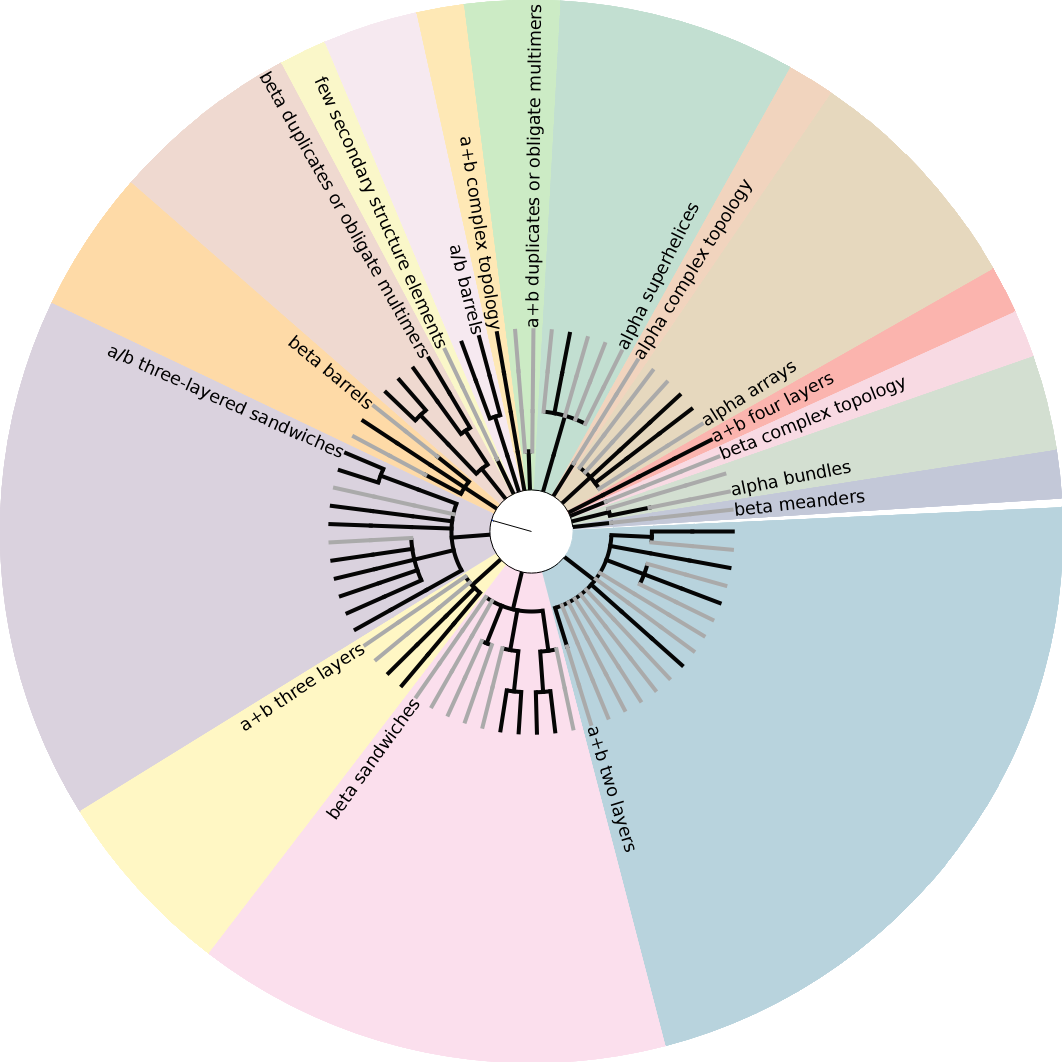
\includegraphics[width=0.50\linewidth]{../draft/Fig/folds_graph.png}
%
    \captionsetup{width=0.8\linewidth}
    \caption{Classification of the test set structures into the lower
    four ECOD structural levels (from the center out): architecture
    (A), possible homology (X), homology (H), and topology (T). The
    names of the architecture types are shown in the outer circle of
    the diagram.
%%% Why do you have two different architecture names in the same A
%%% group? (brown color: ``alpha complex topology'' and ``alpha
%%% arrays'')
    The grey lines denote test set classes that have no
    respective representative in the training set. The black lines
    show the classes that have representatives in both training and
    test sets. We do not show the F-groups because they have litle
    overlap among the training and test sets.
%%% Why not showing the F-groups?
}
%
    \label{Fig:foldsGraph}
\end{figure}
\end{block}

\end{textblock}


\begin{textblock}{39.0}(43.5,6)

\begin{block}{Results}

We assess the performance of our method (3DCNN) using different rank
correlation coefficients, and using the loss criterion, defined as the
deviation of the GDT\_TS of the best decoy from the GDT\_TS of the
decoy with the lowest score:
$$ 
\text{Loss} = \left| \max_i( \textrm{GDT\_TS}(x_i) ) - \textrm{GDT\_TS} [ \textrm{argmin}_i( \textrm{3DCNN}(x_i) ) ] \right|
$$ 

\vspace{0.5cm}
Table \ref{Tbl:TestResults} shows the comparison of our algorithm
(3DCNN) with state-of-the-art methods ProQ2 \cite{ray2012proq2},
VoroMQA \cite{olechnovivc2017voromqa}, Qprob \cite{cao2016protein},
and RWplus \cite{zhang2010novel}.

\begin{table}[H]
\begin{center}
\begin{tabular}{ c | c | c | c | c }
    \multicolumn{5}{ c }{Stage 1} \\ \hline

    QA method & Loss & Pearson & Spearmann & Kendall \\
    \hline
    \textbf{3DCNN}   &0.071 &0.528 &0.414 &0.318 \\
    ProQ2   &0.081 &0.656 &0.534 &0.408 \\
    VoroMQA &0.095 &0.621 &0.504 &0.382 \\
    Qprob   &0.097 &0.631 &0.517 &0.389 \\
    RWplus  &0.128 &0.500 &0.387 &0.291 \\ \hline
    
    \multicolumn{5}{ c }{Stage 2} \\ \hline
    
    ProQ2   &0.058 &0.372 &0.366 &0.256 \\
    \textbf{3DCNN}   &0.067 &0.420 &0.405 &0.285 \\
    Qprob   &0.068 &0.381 &0.387 &0.272 \\
    VoroMQA &0.069 &0.444 &0.437 &0.313 \\ 
    RWplus  &0.095 &0.202 &0.246 &0.175 \\ \hline

\end{tabular}
\vspace{0.25cm}    
    \captionsetup{width=0.8\linewidth}
    \caption {Performance of our method (3DCNN) on the CASP11 dataset
      (Stages 1 and 2), compared to other state-of-the-art QA
      programs. The table shows the absolute, per-target average
      values of the loss and the correlation coefficients.}
    \label{Tbl:TestResults}
\end{center}
\end{table}

\end{block}

\begin{block}{Analysis}
The neural networks are famous for their lack of interpretability. 
Therefore we have to ensure the following:
\begin{itemize}
\item Our model does not overfit 
\item It gives approximatelly the same score for a rotated and translated decoy 
\item It does not rely on some artifacts that can attribute a decoy to a certain contestant, which 
in turn are correlated with the score
\end{itemize}

During the training of the model we augmented the data using random uniform rotations and random translations. 
The Fig. \ref{Fig:DecoysScoreDistribution} shows that the scores under random transformations are distributed approximatelly normally.

To assess the degree of overfitting of our algorithm, we used the classification of targets presented on Fig. \ref{Fig:foldsGraph}
Figure \ref{Fig:LossVsECOD} shows the performance of the algorithms depending on the degree of homology. 
We see, that our algorithm has approximatelly the same performance gains for the homologous proteins as the VoroMQA and ProQ2. 
The algorithm that stands out in this metric is the RWPlus, which seems to be indifferent to the homology. 
However, its performance is also lower than that of the other contenders.

\begin{figure}[H]
\nocaption
    \centering
    \begin{subfigure}[t]{.5\textwidth}
    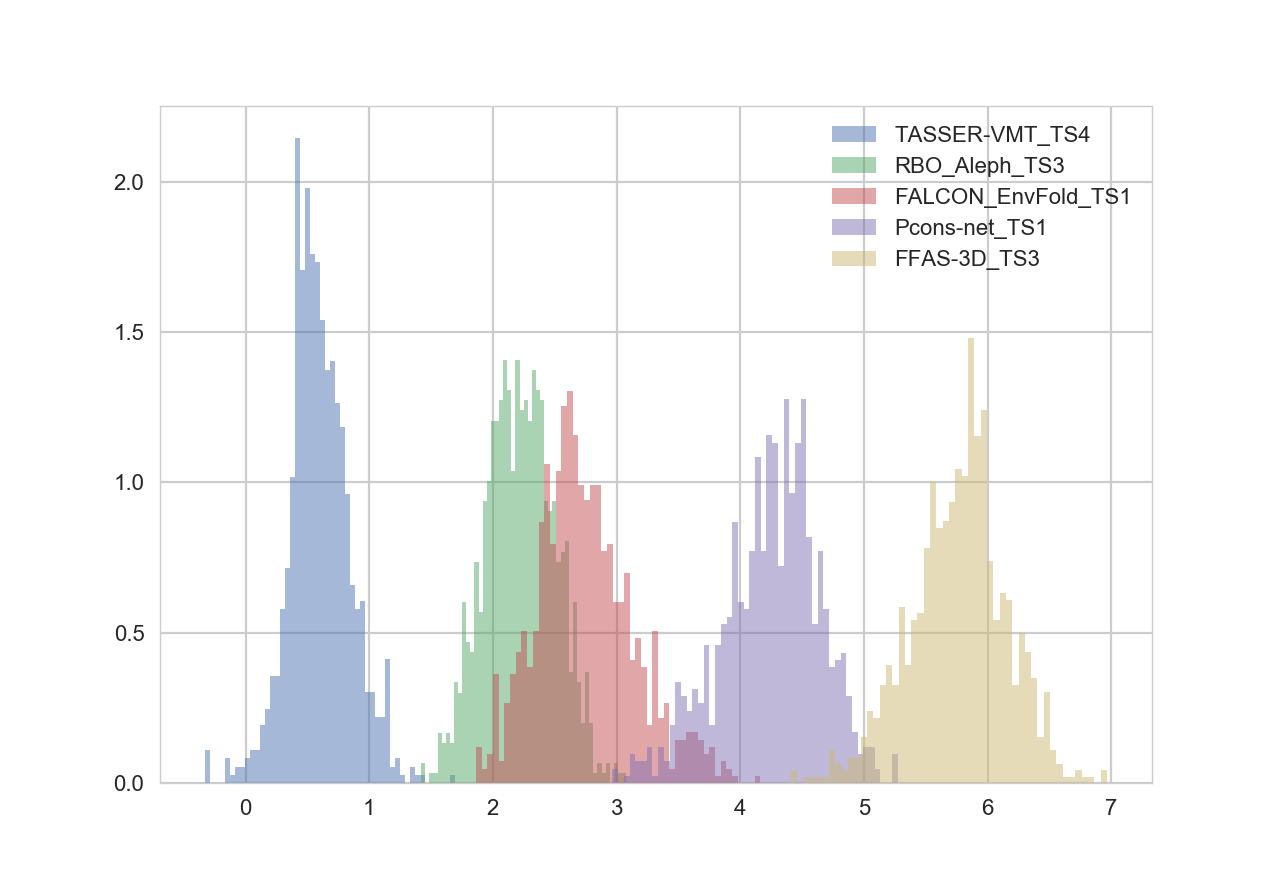
\includegraphics[width=\linewidth]{../draft/Fig/decoys_sampling_dist.png}
    \captionsetup{width=\linewidth}
    \caption{Distributions of scores under random translations and
      rotations of several decoys for target T0832. The names
      arrangement from top to bottom corresponds to the increase of
      the score.}
    \label{Fig:DecoysScoreDistribution}
    \end{subfigure}%
    \begin{subfigure}[t]{.5\textwidth}
    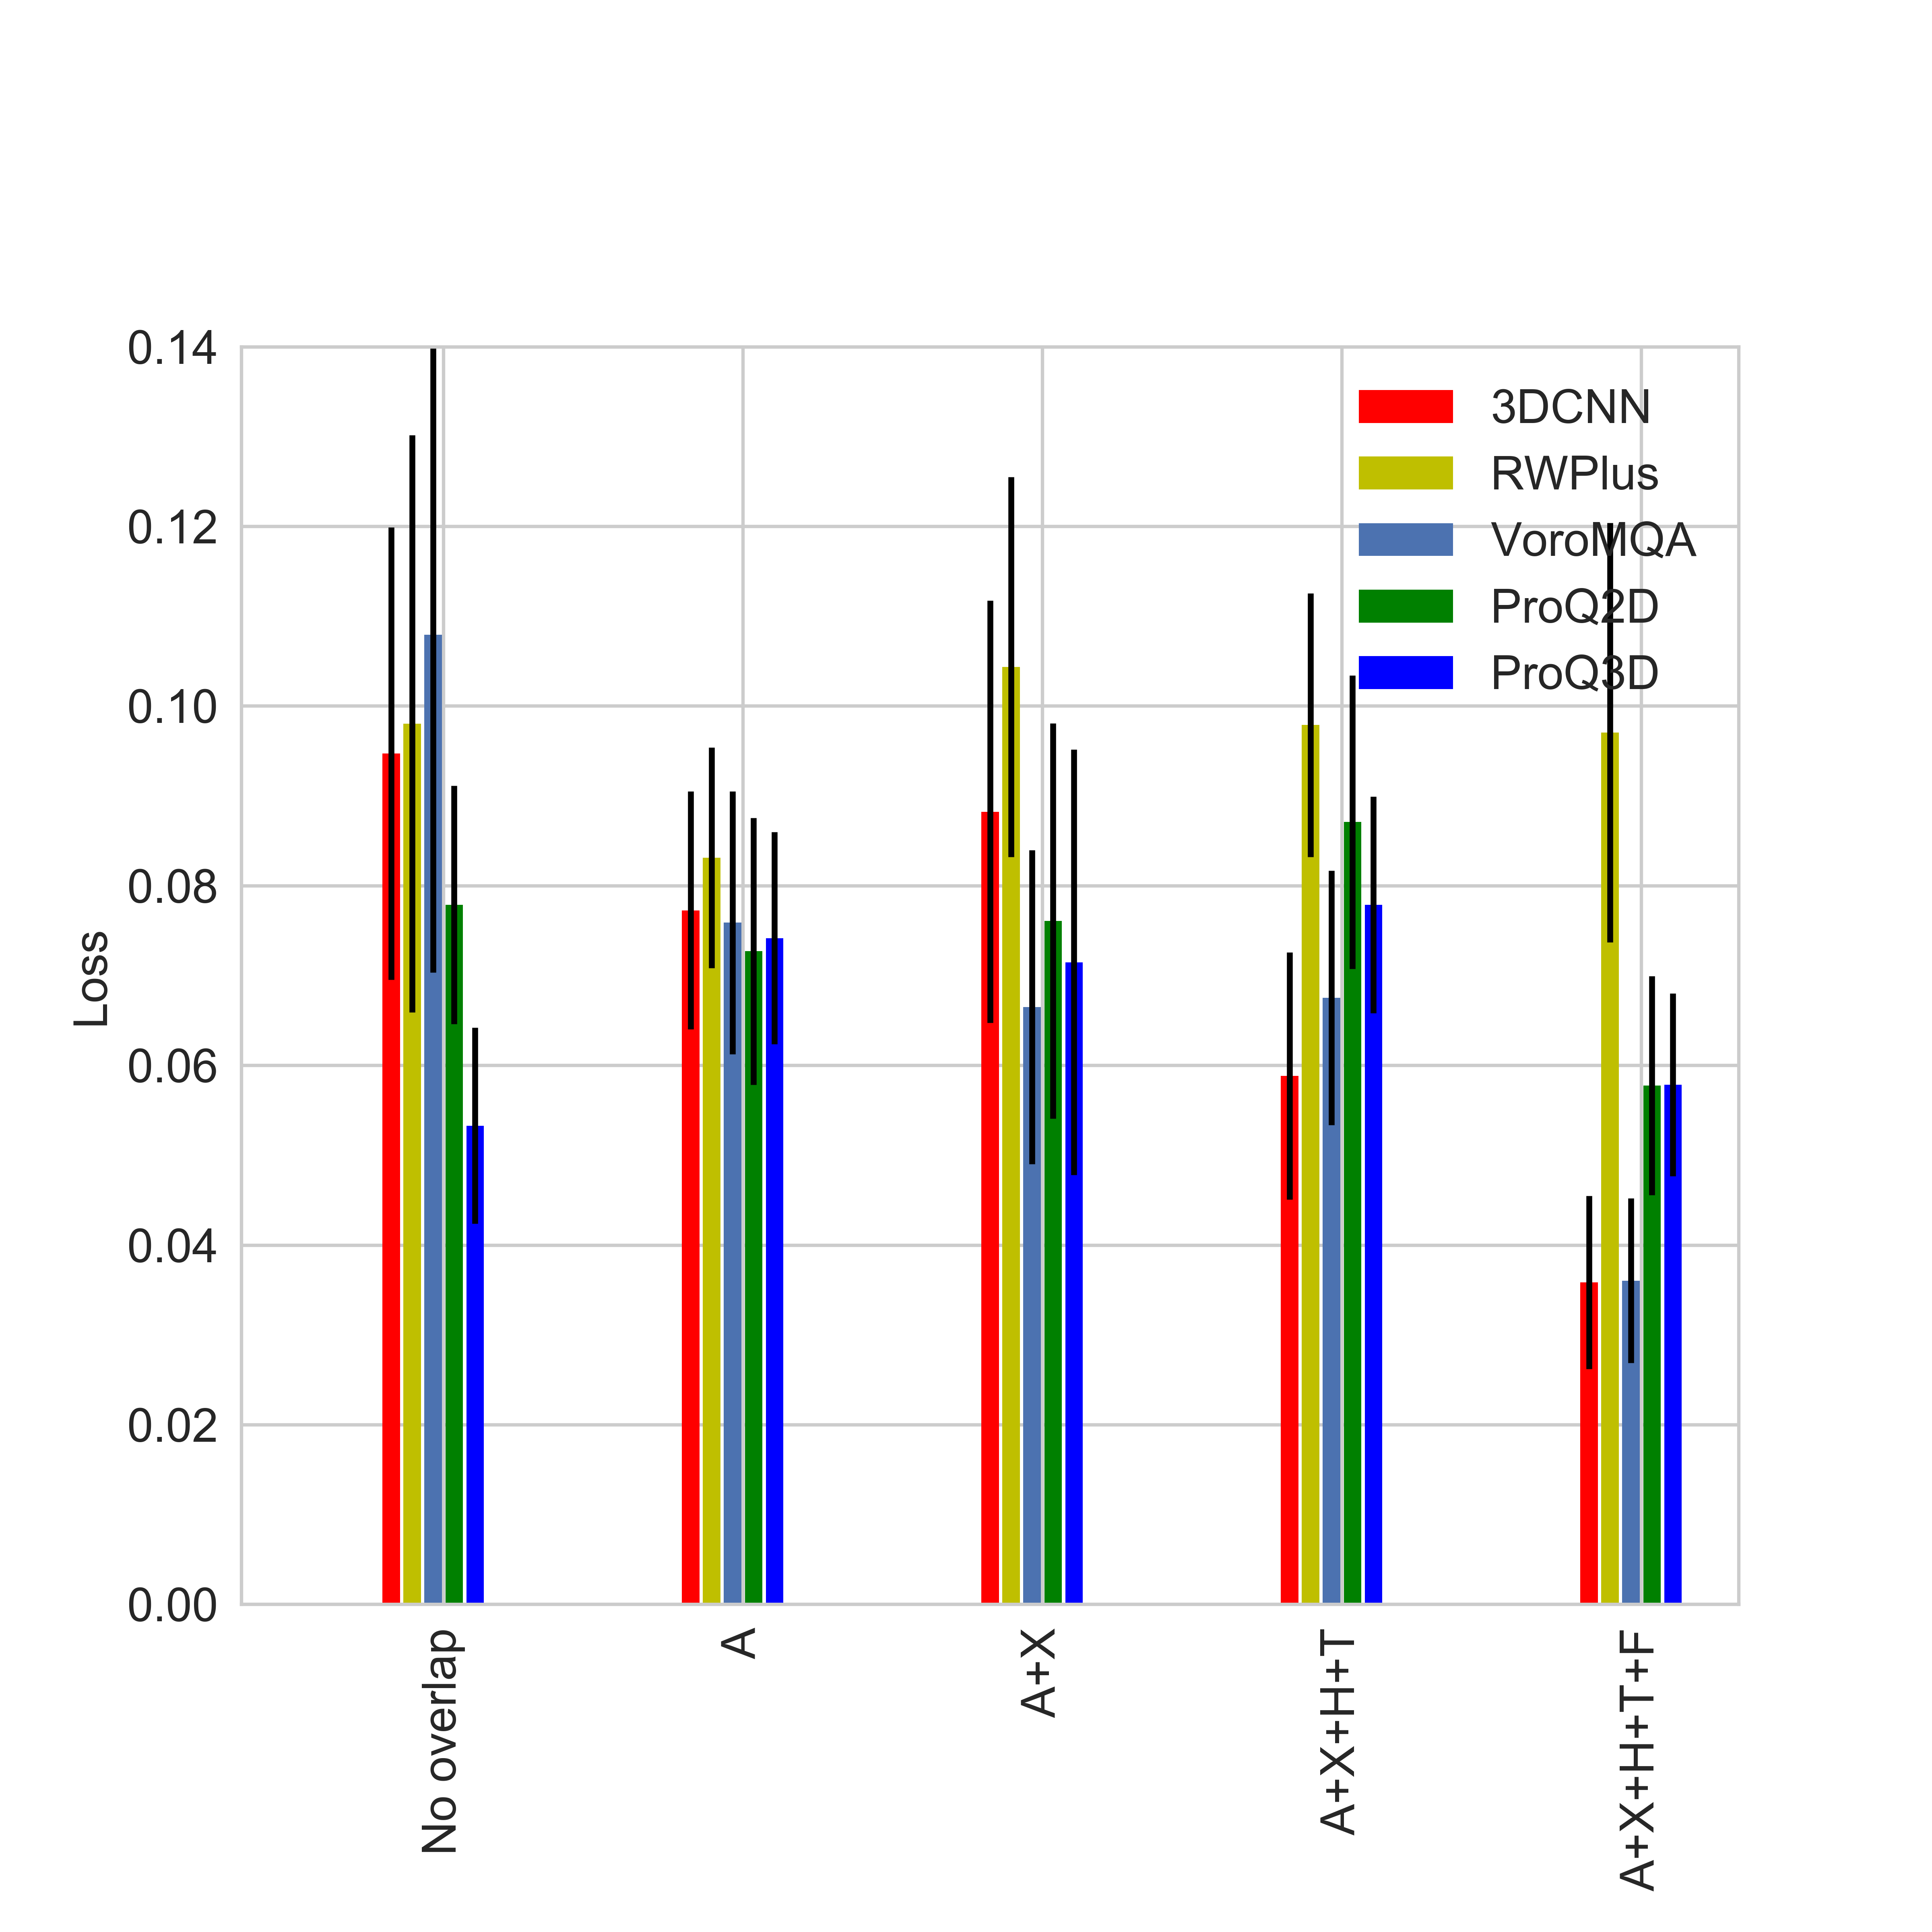
\includegraphics[width=\linewidth]{../draft/Fig/LossVsECOD.png}
    \captionsetup{width=\linewidth}
    \caption{Loss of different QA-algorithms on the subsets of the
      CASP11 test set Stage2. The subsets are chosen according to the
      presense in the training set of the structures classified into
      the same ECOD categories.}
    \label{Fig:LossVsECOD}
    \end{subfigure}
    % \caption{}
\end{figure}

Finally, to ensure that our algorithm does indeed learn from the structural information and not some artifacts we visualized 
the regions that influense the score the most.
We use the GradCAM method proposed by Selvaraju R. \cite{selvaraju2016grad}. 
It outputs the receptive field, that indicate which parts of the input contributes the most to the positive part of the gradient of the network output.
Fig. \ref{Fig:GradCAMT0776_more} shows the projection of the GradCAM output on the heavy atoms of a protein. 
We see that it highlights the regions at the surface of the protein that are likely misfolded.

\begin{figure}[H]
    \centering
    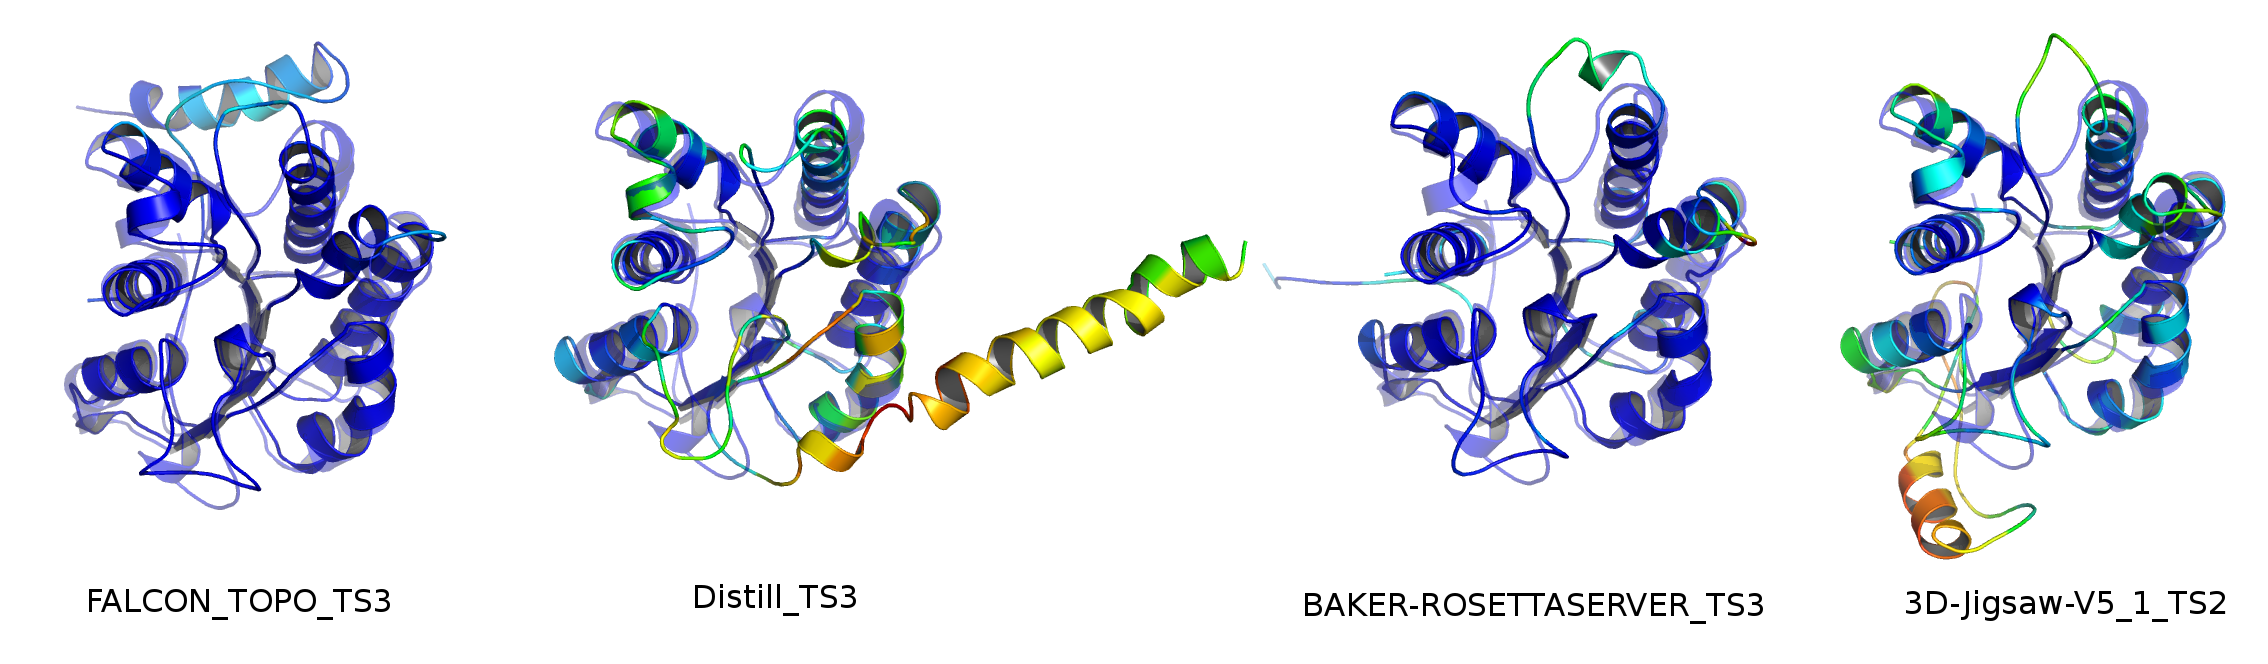
\includegraphics[width=\linewidth]{../draft/Fig/T0776.png}
    \captionsetup{width=0.8\linewidth}
    \caption{The scaled gradient weighted activation maps of the
      network projected onto the atoms of the decoys.  Each decoy is
      aligned to the native structure (shown with the transparent
      cartoon).}
    \label{Fig:GradCAMT0776_more}
\end{figure}

We also verified that the decoys generated by a single algorithm not used in CASP can be successfully ranked by our model.
For this purpose we used 3DRobot dataset \cite{deng20163drobot}. The pearson correlation between the score assigned by 
3DCNN and the GDT\_TS is $0.85$. This indicates, that our algorithm can generalize rather well.

\end{block}




\begin{block}{Acknowledgments}
This research was supported by an NSERC Discovery Grant to G.L.
We thank our collaborators from MILA lab for comments and suggestions.
\end{block}

\begin{block}{References}
{\small
\bibliography{../draft/citations.bib}{}}
\bibliographystyle{ieeetr}
\end{block}

\end{textblock}

\end{frame}
\end{document}
